
\documentclass{beamer}

\usepackage{cmap}                                       % поиск в PDF
\usepackage[T2A]{fontenc}                       % кодировка
\usepackage[utf8]{inputenc}                     % кодировка исходного текста
\usepackage[english,russian]{babel}     % локализация и переносы

\usepackage{graphicx}
\graphicspath{{images/}}

%% \usetheme{Berkeley}
%% \usecolortheme{beaver}
\definecolor {processblue}{cmyk}{0.96,0,0,0}

\usepackage{tikz}
\usetikzlibrary {automata, arrows, positioning}
%% \usepackage{tikz,fullpage}

\logo{\includegraphics[height=0.8cm]{bsu_logo_ru.eps}}
\title{Основы теории скрытых марковских моделей}
\author{Кузьмин А.А.}
\institute[]{\url{http://rfe.bsu.by/}}

\begin{document}

\begin{frame}
  \maketitle
\end{frame}

\section{Содержание}

\begin{frame} \label{cont}
  \frametitle{\insertsection}
  \begin{enumerate}
    \item Понять проблему из-за которой представление сигнала как случайного вектора не достаточно \pause
    \item Понять что из себя представляют \alert{скрытые марковские модели (СММ)} в самом простом случае и из чего они состоят\pause
    \item Познакомиться с тем как ими правильно пользоваться \pause
      $3$ проблемы СММ
  \end{enumerate}
\end{frame}

\section{Пролема с представлением сигнала как случайного вектора}
\begin{frame}
  \frametitle{\insertsection}
  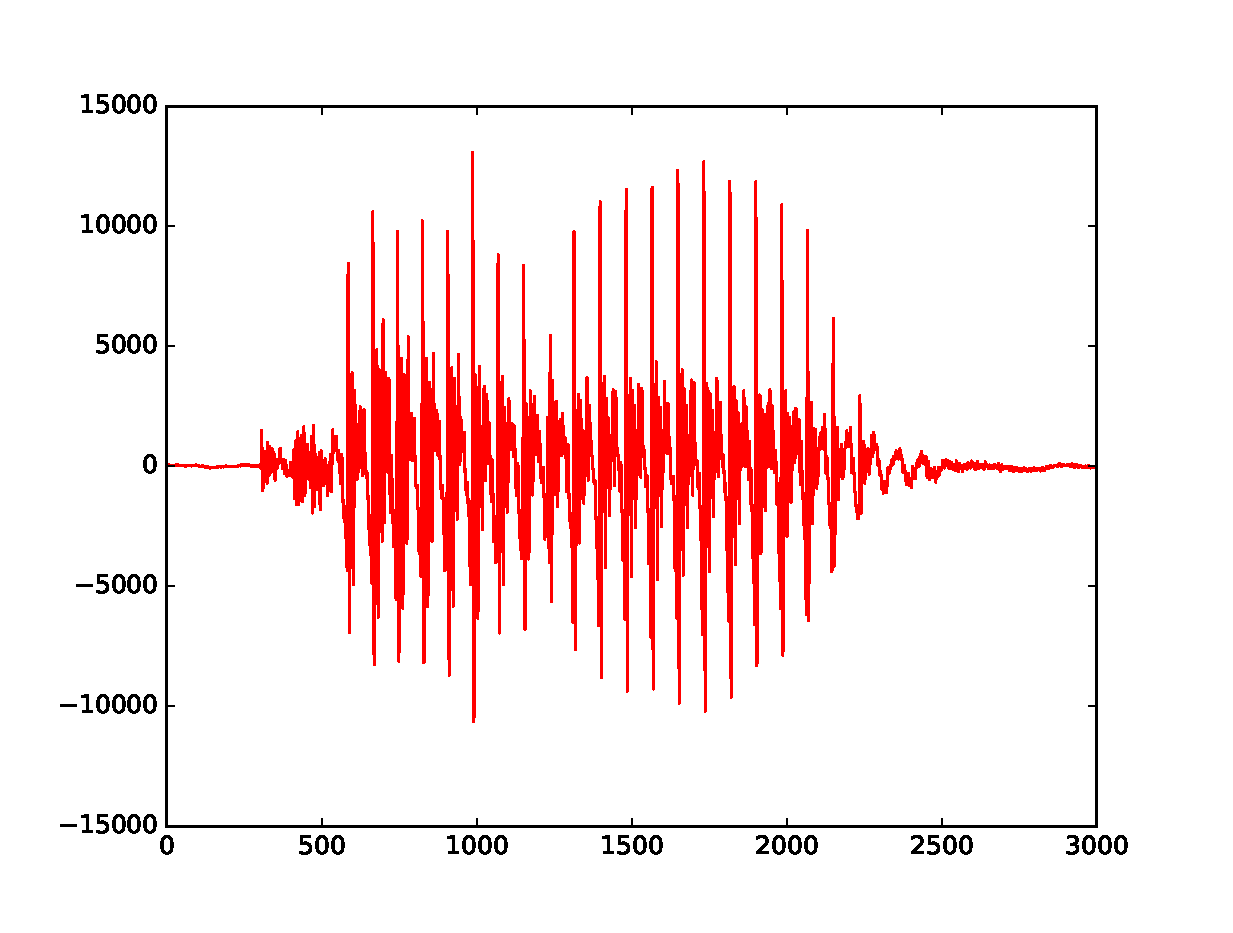
\includegraphics[width=0.8\textwidth]{a_short.eps}
\end{frame}

\section{Пролема с представлением сигнала как случайного вектора}
\begin{frame}
  \frametitle{\insertsection}
  \includegraphics[width=0.8\textwidth]{a_long.eps}
\end{frame}

\section{Пролема с представлением сигнала как случайного вектора}
\begin{frame}
  \frametitle{\insertsection}
  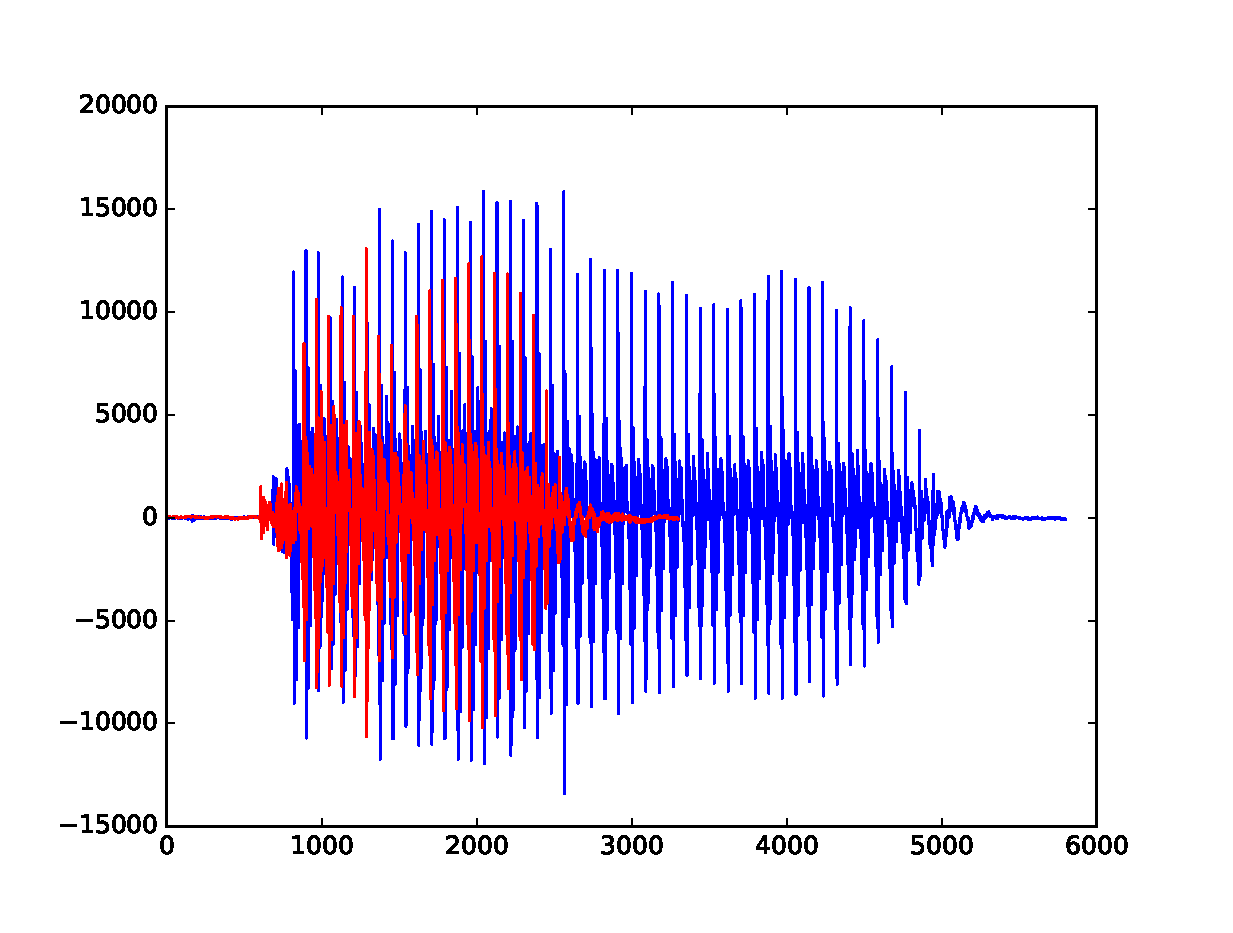
\includegraphics[width=0.8\textwidth]{a_long_short.eps}
\end{frame}

\section{Марковский процесс дискретный по времени}
\subsection{Основные понятия}

%% Будем стараться быть проблема-ориентированными
\begin{frame}
  \frametitle{\insertsection}
  \framesubtitle{Система включающая $N$ состояний $S_1, S_2, \ldots, S_N$}
  %% 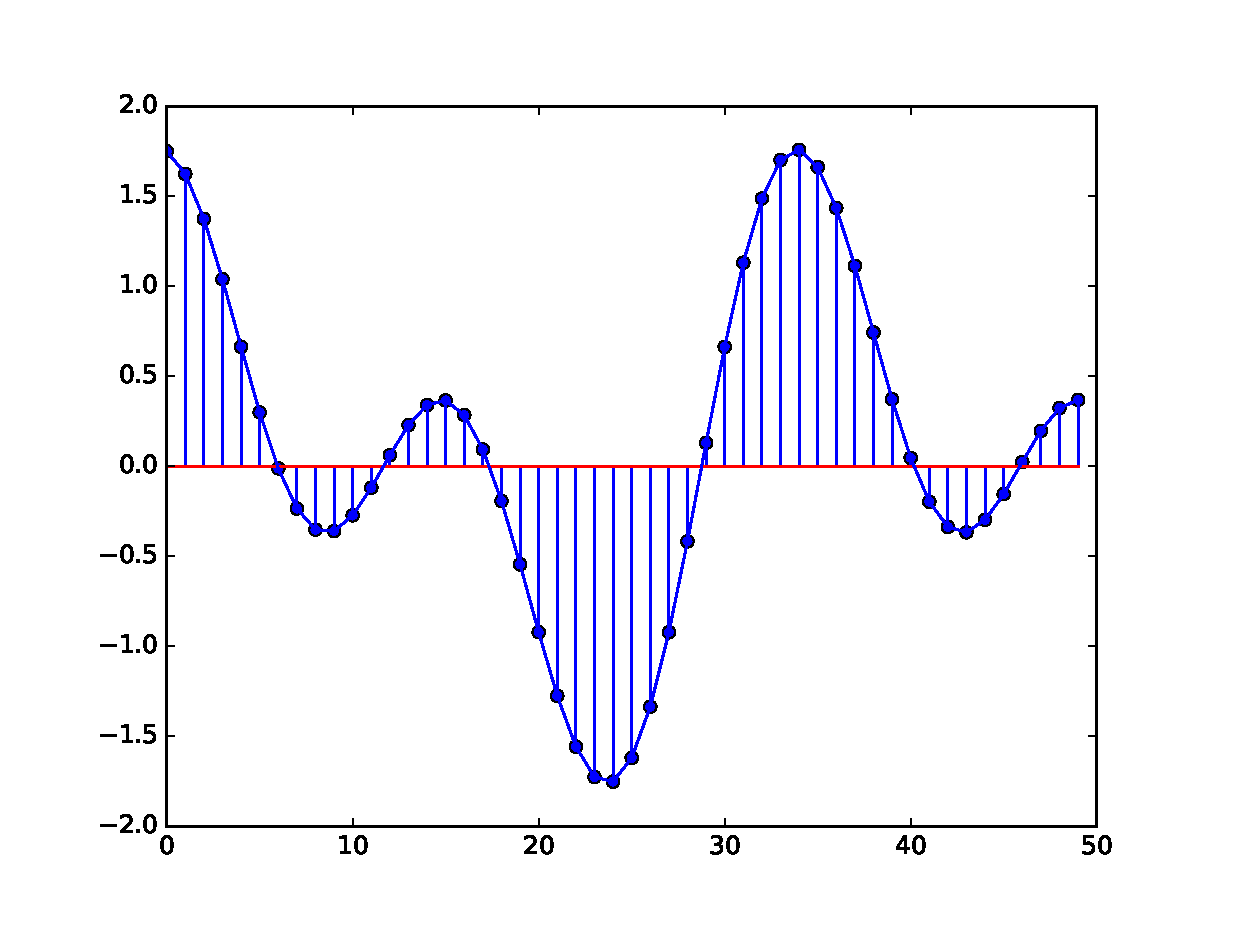
\includegraphics[width=0.8\textwidth]{tovec.eps}

  \begin{figure}
    \centering
    \begin{tikzpicture}[->, >=stealth', auto, node distance =3 cm and 4cm, on grid, semithick]
      \tikzstyle{every state}=[fill=white,draw=black,thick,text=black,scale=0.8]
      \node[state] (C) {$S_3$};
      \node[state] (A) [above left = of C] {$S_1$};
      \node[state] (B) [above right = of C] {$S_2$};
      \path (A) edge [loop left] node {$a_{11}$} (A);
      \path (C) edge [bend left =25] node {$a_{31}$} (A);
      \path (A) edge [bend right = -15] node[below =0.15 cm] {$a_{13}$} (C);
      \path (A) edge [bend left =25] node[above] {$a_{12}$} (B);
      \path (B) edge [bend left =15] node[below =0.15 cm] {$a_{21}$} (A);
      \path (C) edge [bend left =15] node[below =0.15 cm] {$a_{32}$} (B);
      \path (B) edge [bend right = -25] node[below =0.15 cm] {$a_{23}$} (C);
    \end{tikzpicture}
  \end{figure}
\end{frame}

\begin{frame} 
  \frametitle{\insertsection}
    \framesubtitle{\insertsubsection}
  \begin{itemize}
    \item $S_1, S_2, \ldots, S_N$
    \item $t_1, t_2, \ldots$
    \item состояние в момень времени $t$: $q_t$
    \item полное вероятностное описание: $P(q_t = S_i | q_{t - 1} = S_j, q_{t - 2} = S_k, \ldots) = $ \pause $P(q_t = S_i | q_{t - 1} = S_j)$
      \\ для цепи Маркова
      %% Вероятность находится в том или ином состоянии в данный момент
      %% с учетом того в каких состояниях находилась система до этого
  \end{itemize}
\end{frame}

\begin{frame} 
  \frametitle{\insertsection}
    \framesubtitle{\insertsubsection}
  \begin{itemize}
    \item $a_{ij} = P(q_t = S_i | q_{t - 1} = S_j)$ \pause
    \item $a_{ij} \ge 0, \forall i, \forall j$ \pause
    \item $\displaystyle \sum_{j = 1}^{N} a_{ij} = 1$
  \end{itemize}
\end{frame}

\subsection{Конкретный пример}

\begin{frame} 
  \frametitle{\insertsection}
    \framesubtitle{\insertsubsection}
  \begin{itemize}
    \item $S_1$: ``\textit{Снег}'' (``\textit{Дождь}'')
    \item $S_2$: ``\textit{Пасмурно}''
    \item $S_3$: ``\textit{Солнечно}''
  \end{itemize}
  \begin{equation*}
    A = \{a_{ij}\} =
    \begin{bmatrix}
      0.4 & 0.3 & 0.3 \\
      0.2 & 0.6 & 0.2 \\
      0.1 & 0.1 & 0.8 \\
    \end{bmatrix}
  \end{equation*}
\end{frame}

\begin{frame} 
  \frametitle{\insertsection}
    \framesubtitle{\insertsubsection}
    \begin{figure}
    \centering
    \begin{tikzpicture}[->, >=stealth', auto, node distance =3 cm and 4cm, on grid, semithick]
      \tikzstyle{every state}=[fill=white,draw=black,thick,text=black,scale=0.8]
      \node[state] (C) {$S_3$};
      \node[state] (A) [above left = of C] {$S_1$};
      \node[state] (B) [above right = of C] {$S_2$};
      \path (A) edge [loop left] node {$0.4$} (A);
      \path (B) edge [loop right] node {$0.4$} (B);
      \path (C) edge [loop below] node {$0.4$} (C);
      \path (C) edge [bend left =25] node {$0.1$} (A);
      \path (A) edge [bend right = -15] node[below =0.15 cm] {$0.3$} (C);
      \path (A) edge [bend left =25] node[above] {$0.3$} (B);
      \path (B) edge [bend left =15] node[below =0.15 cm] {$0.2$} (A);
      \path (C) edge [bend left =15] node[below =0.15 cm] {$0.1$} (B);
      \path (B) edge [bend right = -25] node[below =0.15 cm] {$0.8$} (C);
    \end{tikzpicture}
  \end{figure}
\end{frame}

\begin{frame} \label{example_begin}
  \frametitle{\insertsection}
  \framesubtitle{\insertsubsection}
  Какова вероятность такого прогноза на неделю: \\
  ``\textit{\small{солнечно-солнечно-дождь-дождь-солнечно-пасмурно-солнечно}}''\\
  Формально: $O = S_3, S_3, S_1, S_1, S_3, S_2, S_3$ \pause

  \begin{eqnarray*}
    P(O | \text{Model}) & = & P(S_3, S_3, S_1, S_1, S_3, S_2, S_3 | \text{Model})\\
    & = & P(S_3) \cdot P(S_3|S_3) \cdot P(S_1|S_3) \cdot P(S_1|S_1) \cdot \\
    && P(S_3|S_1) \cdot P(S_2|S_3) \cdot P(S_3|P_2) \\
    & = & \sum_{i = 1}^{n}\sum_{j = 1}^{n} h_{ij}(x_i - m_i)(x_j - m_j) \\
    & = & \pi_3 \cdot a_{33} \cdot a_{13} \cdot a_{11} \cdot a_{31}\cdot a_{23} \cdot a_{32}
  \end{eqnarray*}
  где $\pi_i = P(q_1 = S_i)$
\end{frame}

\begin{frame} \label{example_begin}
  \frametitle{\insertsection}
  \framesubtitle{\insertsubsection}
  Какова вероятность такого прогноза на неделю: \\
  ``\textit{\small{солнечно-солнечно-дождь-дождь-солнечно-пасмурно-солнечно}}''\\
  Формально: $O = S_3, S_3, S_1, S_1, S_3, S_2, S_3$

  \begin{eqnarray*}
    P(O | \text{Model}) & = & 1 \cdot (0.8)(0.1)(0.4)(0.3)(0.1)(0.2) \\
    & = & 1.920 \times 10^{-4}
  \end{eqnarray*}
\end{frame}


\section{Скрытые марковские модели}

\subsection{Предварительные примеры. Монеты}

\begin{frame}
  \frametitle{\insertsection}
  \framesubtitle{\insertsubsection}
  \begin{figure}
    \begin{center}
      \begin{tikzpicture}[->, >=stealth', auto, semithick, node distance=3cm]
        \tikzstyle{every state}=[fill=white,draw=black,thick,text=black,scale=1]
        \node[state]    (A)                     {$1$};
        \node[state]    (B)[right of=A]   {$2$};
        \path
        (A) edge[loop left]     node{$P(H)$}         (A)
        edge[bend left]     node{$1 - P(H)$}     (B)
        (B) edge[loop right]    node{$1 - P(H)$}      (B)
        edge[bend left,above]     node{$P(H)$}         (A);
      \end{tikzpicture}
    \end{center}  
  \end{figure}
  \begin{equation*}
    \begin{matrix}
      O & = & H & H & T & H & T & T & H & \ldots \\
      S & = & 1 & 1 & 2 & 1 & 2 & 2 & 1 & \ldots
    \end{matrix}
  \end{equation*}
\end{frame}

\begin{frame}
  \frametitle{\insertsection}
  \framesubtitle{\insertsubsection}
  \begin{figure}
    \begin{center}
      \begin{tikzpicture}[->, >=stealth', auto, semithick, node distance=3cm]
        \tikzstyle{every state}=[fill=white,draw=black,thick,text=black,scale=1]
        \node[state]    (A)                     {$1$};
        \node[state]    (B)[right of=A]   {$2$};
        \path
        (A) edge[loop left]     node{$a_{11}$}         (A)
        edge[bend left]     node{$1 - a_{11}$}     (B)
        (B) edge[loop right]    node{$a_{22}$}      (B)
        edge[bend left,above]     node{$1 - a_{22}$}         (A);
      \end{tikzpicture}
    \end{center}  
  \end{figure}

  \begin{equation*}
    \begin{matrix}
      P(H) = P_1     & P(H) = P_2 \\
      P(T) = 1 - P_1 & P(T) = 1 - P_2
    \end{matrix}
  \end{equation*}
  
  \begin{equation*}
    \begin{matrix}
      O & = & H & H & T & H & T & T & H & \ldots \\
      S & = & 2 & 1 & 2 & 2 & 1 & 1 & 1 & \ldots
    \end{matrix}
  \end{equation*}
\end{frame}

\begin{frame} 
  \frametitle{\insertsection}
    \framesubtitle{\insertsubsection}
    \begin{figure}
    \centering
    \begin{tikzpicture}[->, >=stealth', auto, node distance =2 cm and 3cm, on grid, semithick]
      \tikzstyle{every state}=[fill=white,draw=black,thick,text=black,scale=0.8]
      \node[state] (C) {$3$};
      \node[state] (A) [above left = of C] {$1$};
      \node[state] (B) [above right = of C] {$2$};
      \path (A) edge [loop left] node {$a_{11}$} (A);
      \path (B) edge [loop right] node {$a_{22}$} (B);
      \path (C) edge [loop below] node {$a_{33}$} (C);
      \path (C) edge [bend left =25] node {$a_{31}$} (A);
      \path (A) edge [bend right = -15] node[below =0.15 cm] {$a_{13}$} (C);
      \path (A) edge [bend left =25] node[above] {$a_{12}$} (B);
      \path (B) edge [bend left =15] node[below =0.15 cm] {$a_{21}$} (A);
      \path (C) edge [bend left =15] node[below =0.15 cm] {$a_{32}$} (B);
      \path (B) edge [bend right = -25] node[below =0.15 cm] {$a_{23}$} (C);
    \end{tikzpicture}
    \end{figure}

    $P(H) = P_1 \qquad P(H) = P_2  \qquad P(H) = P_3 $ \\
    $ P(T) = 1 - P_1 \qquad P(T) = 1 - P_2 \qquad P(T) = 1 - P_3 $

    $\displaystyle
    \begin{matrix}
      O & = & H & H & T & H & T & T & H & \ldots \\
      S & = & 3 & 1 & 2 & 3 & 1 & 1 & 2 & \ldots
    \end{matrix}
    $

\end{frame}

\subsection{Предварительные примеры. Урны с шарами}

\begin{frame} 
  \frametitle{\insertsection}
  \framesubtitle{\insertsubsection}

  \begin{table}
    \begin{tabular}{ccc}
      КАРЗИНА $1$ & КАРЗИНА $2$ & КАРЗИНА $3$ \\
      $P(\text{RED}) = b_1(1)$ & $P(\text{RED}) = b_2(1)$ & $P(\text{RED}) = b_3(1)$ \\
      $P(\text{BLUE}) = b_1(2)$ & $P(\text{BLUE}) = b_2(2)$ & $P(\text{BLUE}) = b_3(2)$ \\
      $P(\text{GREEN}) = b_1(3)$ & $P(\text{GREEN}) = b_2(3)$ & $P(\text{GREEN}) = b_3(3)$ \\
      \vdots & \vdots & \vdots \\
      $P(\text{BLACK}) = b_1(M)$ & $P(\text{BLACK}) = b_2(M)$ & $P(\text{BLACK}) = b_3(M)$ \\ 
    \end{tabular}
  \end{table}
  
  \begin{equation*}
  O = \text{GREEN},  \text{BLACK}, \text{BLUE}, \text{RED}, \text{RED}, \ldots, \text{BLUE}    
  \end{equation*}

\end{frame}

\subsection{Ингридиенты}

\begin{frame} 
  \frametitle{\insertsection}
  \framesubtitle{\insertsubsection}
  %% Любая теория начинается с базовых понятий (или с проблемы)
  \begin{enumerate}
  \item Количество состояний: $N$ \pause
  \item Множество наблюдаемых значений $\{v_k\}$ с количеством элементов $M$ \pause
  \item Матрица вероятностей перехода из одного состояния в другу: \\
    $A = \{a_{ij}\}$, где $a_{ij} = P(q_t = S_i | q_{t - 1} = S_j)$ \pause
  \item Вероятность получить то или иное наблюдение при условии нахождения в определенном состоянии: \\
    $B = {b_i(k)}$, где $b_i(k) = P(O_t = v_k | q_t = S_i)$, \\
    $1 \le i \le N$, $1 \le k \le M$ \pause
    \item Начальные вероятности: $\pi_i = P(p_1 = S_i)$, $1 \le i \le M$
  \end{enumerate}

  \pause
  \begin{equation*}
    \lambda = {A, B, \pi}
  \end{equation*}

\end{frame}

\section{Три базовые проблемы СММ}
%% Или как пользоваться СММ
\subsection{Проблема 1}
%% Задачка, которую надо решить поскольку очень нужен ответ

\begin{frame} 
  \frametitle{\insertsection}
  \framesubtitle{\insertsubsection}
  \begin{itemize}
  \item Дана последовательность наблюдений: $O = O_1, O_2, \ldots, O_T$
  \item Есть модель $\lambda = \{A, B, \pi \}$
  \item Какова вероятность того что последовательность была сгенерирована данной моделью: \\
    $P(O | \lambda) = ?$
  \end{itemize}
\end{frame}

\subsection{Проблема 2}

\begin{frame} 
  \frametitle{\insertsection}
  \framesubtitle{\insertsubsection}
  \begin{itemize}
  \item Дана последовательность наблюдений: $O = O_1, O_2, \ldots, O_T$
  \item Есть модель $\lambda = \{A, B, \pi \}$
  \item Какова последовательность состояний модели $Q = q_1, q_2, \ldots, q_T$, которая наилучшим (в некотром смысле) образом соответствует $O$?
  \end{itemize}
\end{frame}


\section{Наиболее вероятная последовательность состояний модели}

\section{Оптимальные значения параметров модели}
\subsection{Расчет значений параметров для случая непрерывного времени}

\section{Виды скрытых марковских моделей}

\section{Масштабиование значений вероятностей}


\end{document}
